\section{Introduction}

Assessing the perceptual quality of synthetic speech is crucial for guiding the development and refinement of speech generation models \citep{valentini2018speech}. The rapid progress of text-to-speech (TTS) and generative audio models has dramatically improved the naturalness and expressiveness of synthetic speech \citep{wang2025spark, xu2025qwen2}, but also created new challenges for evaluating speech quality at scale \citep{lo2019mosnet, huang2022voicemos}.


%=======主图
\begin{figure}[tbh]
\setlength{\abovecaptionskip}{-2pt}
\begin{center}
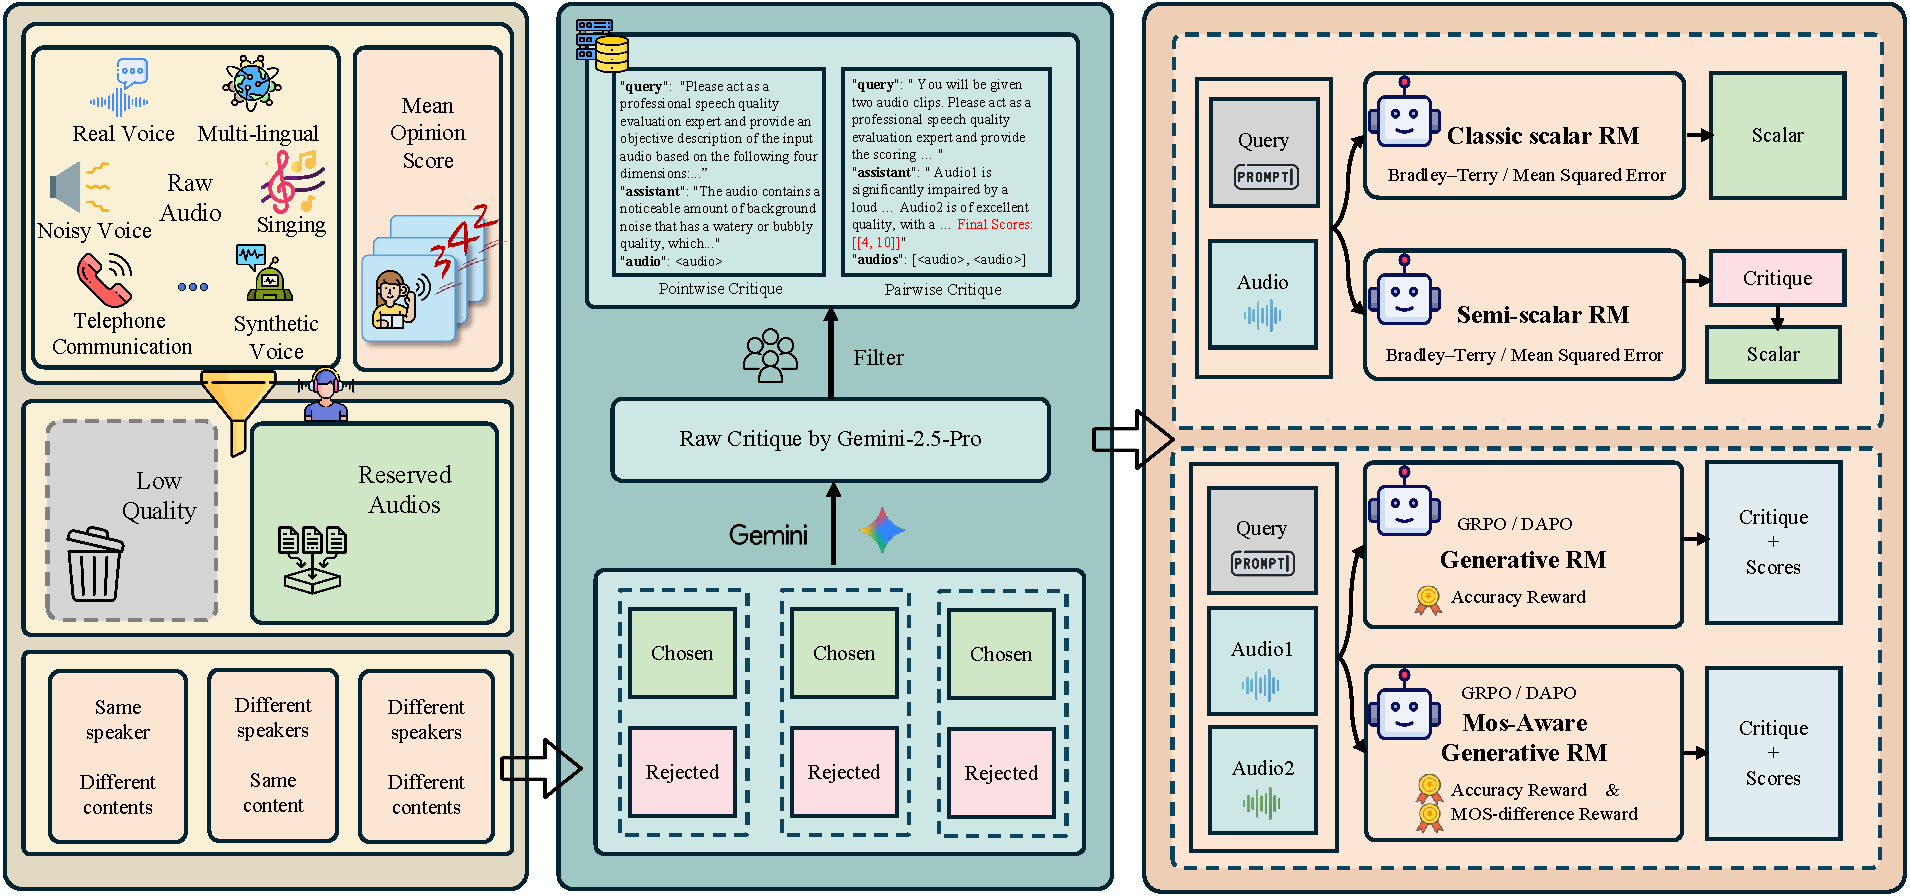
\includegraphics[width=\textwidth]{pictures/MOS-RMBench.pdf}
\end{center}
\caption{Overview of MOS-RMBench. Data from multiple MOS datasets are filtered and grouped, then converted into pairwise comparisons with natural-language critiques generated by Gemini-2.5-Pro. The resulting dataset supports training and evaluation of reward models in a consistent and reproducible setting.}
\label{fig:mos-rmbench}
\vskip -0.1in
\end{figure}



However, perceptual quality assessment has traditionally relied on human subjective ratings such as the Mean Opinion Score (MOS) \citep{international1996methods}, which depend on manual annotations and often suffer from inconsistent rating standards and poor reproducibility. MOS-based evaluation asks listeners to rate the quality of speech samples on a fixed scale and averages the scores to produce ground-truth labels. While this approach has been the de facto standard for decades \citep{international1996methods}, it is expensive to collect, subject to human variability, and difficult to scale for modern systems that generate massive amounts of data \citep{mittag2019non}. Furthermore, variations in listener populations and rating procedures lead to inconsistent subjective standards, hindering reproducibility and cross-dataset comparison \citep{pieper2024alignnet}.

To address these limitations, we introduce MOS-RMBench (see Figure \ref{fig:mos-rmbench}), a unified benchmark that reformulates diverse MOS datasets into a preference-comparison setting, enabling rigorous evaluation across different datasets. By transforming MOS scores into pairwise preference labels, MOS-RMBench eliminates scale inconsistencies and allows models to be trained and evaluated under a consistent comparison framework.

Building on MOS-RMBench, we systematically construct and evaluate three paradigms for reward modeling: scalar reward models, semi-scalar reward models, and generative reward models (GRMs). First, we find that scalar models achieve the strongest overall performance, consistently exceeding 74\% accuracy and reaching around 80\% on average across both in-domain and out-of-domain (OOD) datasets, establishing a solid baseline for future work. Second, we observe that most models perform considerably worse on synthetic speech datasets such as SOMOS \citep{somos} and VMC'23 \citep{vmc23} compared to human speech, underscoring a persistent domain gap. Finally, although all models struggle on pairs with very small MOS differences, they perform very well when the MOS gap is large, indicating that the key challenge lies in fine-grained quality discrimination.

To improve performance on these challenging pairs, we propose a MOS-aware GRM that augments the standard correctness-based reward with an additional MOS-difference–based reward, enabling the model to adaptively scale rewards according to the difficulty of each sample pair. Experimental results show that the MOS-aware GRM consistently improves performance across all evaluated datasets, with accuracy gains exceeding 3\% on samples with particularly similar speech quality.

We hope this work will establish both a benchmark and a methodological framework to foster more rigorous and scalable research in automatic speech quality assessment. Overall, our contributions are threefold:
\begin{enumerate}
\setlength\parskip{0em}
    \item We present MOS-RMBench, the first unified benchmark that reformulates heterogeneous MOS datasets into a consistent preference-comparison framework, enabling rigorous cross-dataset evaluation.
    \item We conduct a systematic evaluation of reward modeling paradigms, comparing scalar, semi-scalar, and generative models across diverse speech domains, and providing insights into their relative strengths and weaknesses.
    \item We introduce a MOS-aware GRM that adaptively scales pairwise rewards based on MOS differences, achieving measurable improvements in fine-grained speech quality discrimination.
\end{enumerate}